\documentclass[UTF8,a4paper,11pt]{ctexart}

\usepackage[a4paper,margin=18mm,headheight=15pt]{geometry}
\usepackage{graphicx}
\usepackage{booktabs}
\usepackage{tabularx}
\usepackage{array}
\usepackage{xcolor}
\usepackage{tikz}
\usepackage{fancyhdr}
\usepackage{hyperref}
\usepackage{enumitem}

\definecolor{navy}{HTML}{18324B}
\definecolor{teal}{HTML}{0E7490}
\definecolor{green}{HTML}{166534}
\definecolor{amber}{HTML}{A16207}
\definecolor{red}{HTML}{991B1B}
\definecolor{soft}{HTML}{F2F5F7}
\definecolor{linegray}{HTML}{CBD5E1}

\setCJKmainfont{Noto Serif CJK SC}
\setCJKsansfont{Noto Sans CJK SC}
\setmainfont{DejaVu Serif}
\setsansfont{DejaVu Sans}

\hypersetup{colorlinks=true,linkcolor=navy,urlcolor=teal}
\setlist{nosep,leftmargin=1.7em}
\setlength{\parindent}{0pt}
\setlength{\parskip}{0.55em}
\renewcommand{\arraystretch}{1.2}

\pagestyle{fancy}
\fancyhf{}
\lhead{Full Engineering Board V2}
\rhead{PCB 与系统规格说明}
\cfoot{\thepage}
\renewcommand{\headrulewidth}{0.4pt}

\newcommand{\statusbox}[3]{%
  \begin{tikzpicture}
    \node[rounded corners=2pt, draw=#1!45!black, fill=#1!8, inner sep=7pt, text width=0.88\linewidth] {\textbf{#2}\par #3};
  \end{tikzpicture}%
}

\begin{document}

\begin{titlepage}
  \vspace*{8mm}
  {\color{navy}\fontsize{28}{34}\selectfont\bfseries Full Engineering Board V2\par}
  \vspace{3mm}
  {\color{teal}\fontsize{18}{24}\selectfont PCB 效果与目标差距说明\par}
  \vspace{10mm}
  \rule{\linewidth}{1.2pt}
  \vspace{8mm}
  \begin{minipage}{0.53\linewidth}
    这份说明把产品目标和当前板子放在一起看：哪些指标已经有证据，哪些还只是要求，哪些地方需要回到版图和仿真里补。\par

    产品目标是 50 mm x 50 mm 的灰板，透明 PP 外壳加 1.6 mm FR4 基板，正面放线圈、直通线、耦合段和 10 kΩ 识别链，背面整片接地。仓库里的 Full V2 目前仍是 50 mm x 60 mm 的工程候选，使用 V2 T-cell 加矩形 Patch，正好可以用来对照差距。

    先把边界说清楚：当前版图已经通过 PCB 工程检查，但还不是新规格的制造冻结版。加载工件的电磁结果也还没有收敛到可以谈吸收功率的程度。
  \end{minipage}
  \hfill
  \begin{minipage}{0.40\linewidth}
    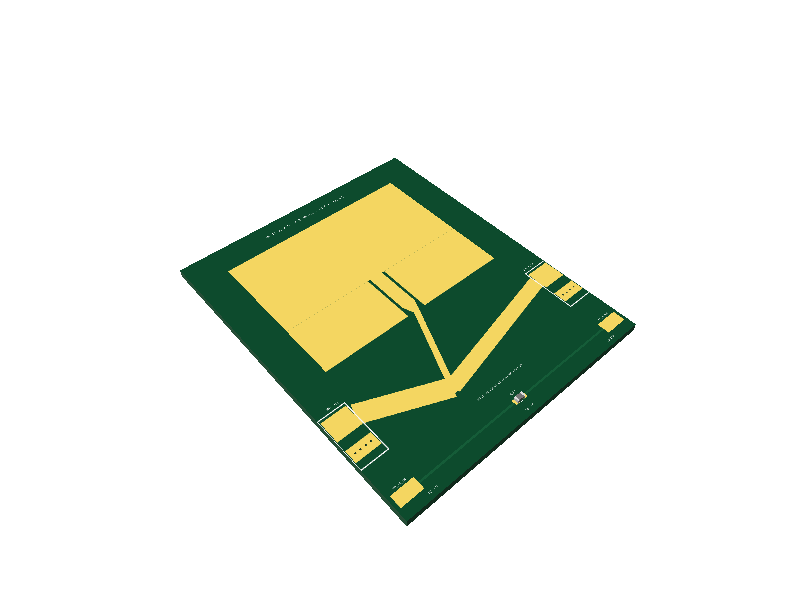
\includegraphics[width=\linewidth]{assets/full-v2-3d.png}
    \vspace{1mm}
    {\footnotesize Full V2 当前 3D 预览。金色区域是顶层 RF 铜，底层连续地平面在该视角下不可见。}
  \end{minipage}

  \vfill
  \statusbox{amber}{当前一句话结论}{Full V2 的空载 RF 筛选已经过关，但 50 x 50 mm 灰板、桥接件和 5/25/100 板功率均匀性还没有在同一个模型里闭合。}
  \par\vspace{8mm}
  \begin{center}{\small 日期：2026-09-22\quad 版本：V1\par}\end{center}
\end{titlepage}

\section{先看结论}

\begin{tabularx}{\linewidth}{>{\bfseries}p{29mm} X >{\raggedleft\arraybackslash}p{22mm}}
\toprule
项目 & 当前证据 & 状态 \\
\midrule
产品灰板规格 & 目标为 50 mm x 50 mm，透明 PP 外壳 + 1.6 mm FR4，背面整片接地 & \textcolor{amber}{待同步} \\
当前板框与走线 & 现有 Full V2 是 50 mm x 60 mm，RF、Patch、ID 链已落版 & \textcolor{amber}{候选} \\
PCB 工程检查 & netlist、placement、走线长度、routing difficulty、build、shorts 均通过；shorts = 0 & \textcolor{green}{已完成} \\
空载 RF screen & fast/open: S11 = -19.34 dB，S21 = -12.49 dB，VSWR = 1.242 & \textcolor{green}{通过} \\
ID RF 影响 & off/open/10 kΩ 在 2.45 GHz 的变化很小 & \textcolor{green}{可忽略} \\
加载工件 & 已建模，但 5 mm gap 的端口时窗只有 0.182 ns，跨 profile 不稳定 & \textcolor{red}{未闭合} \\
组态功率目标 & 单组最大输入 500 W；1-100 板，每板 5-8 W，偏差不超过 +/-25\% & \textcolor{red}{未验证} \\
制造冻结 & RF1 边缘余量只有 0.2 mm，器件 courtyard 和部分 pin 属性仍缺失 & \textcolor{amber}{待处理} \\
\bottomrule
\end{tabularx}

\section{这块 PCB 到底放了什么}

新规格里的灰板是 50 mm x 50 mm。透明 PP 外壳负责保护，1.6 mm FR4 负责承载铜箔，背面是一整片地。正面需要同时放方形螺旋线圈、直通线、耦合段和识别走线；识别走线串接 10 kΩ 电阻。

仓库里的当前 Full V2 还不是这套最终拓扑。它采用左右 RF 磁吸接触、V2 T-cell、分支馈电和矩形 inset-fed Patch，底部另放 TP\_ID\_IN - 10 kΩ / 0603 - TP\_ID\_OUT。这个版本已经能检查 launch、回流、Patch 和 ID 支路的相互影响，但它不能直接证明方形螺旋线圈版本的取能均匀性。

图中左右两侧是 RF 接触区，每个信号接触旁边都有 GND 接触和回流过孔。信号进入后先经过 pad transition，再进入 V2 T-cell。T 点一路继续到 RF OUT，另一路向上接到 Patch。RF 仿真默认保留 ID 铜线，把电阻间隙当作开路；另有显式 10 kΩ 版本用于抽查。

\begin{figure}[ht]
  \centering
  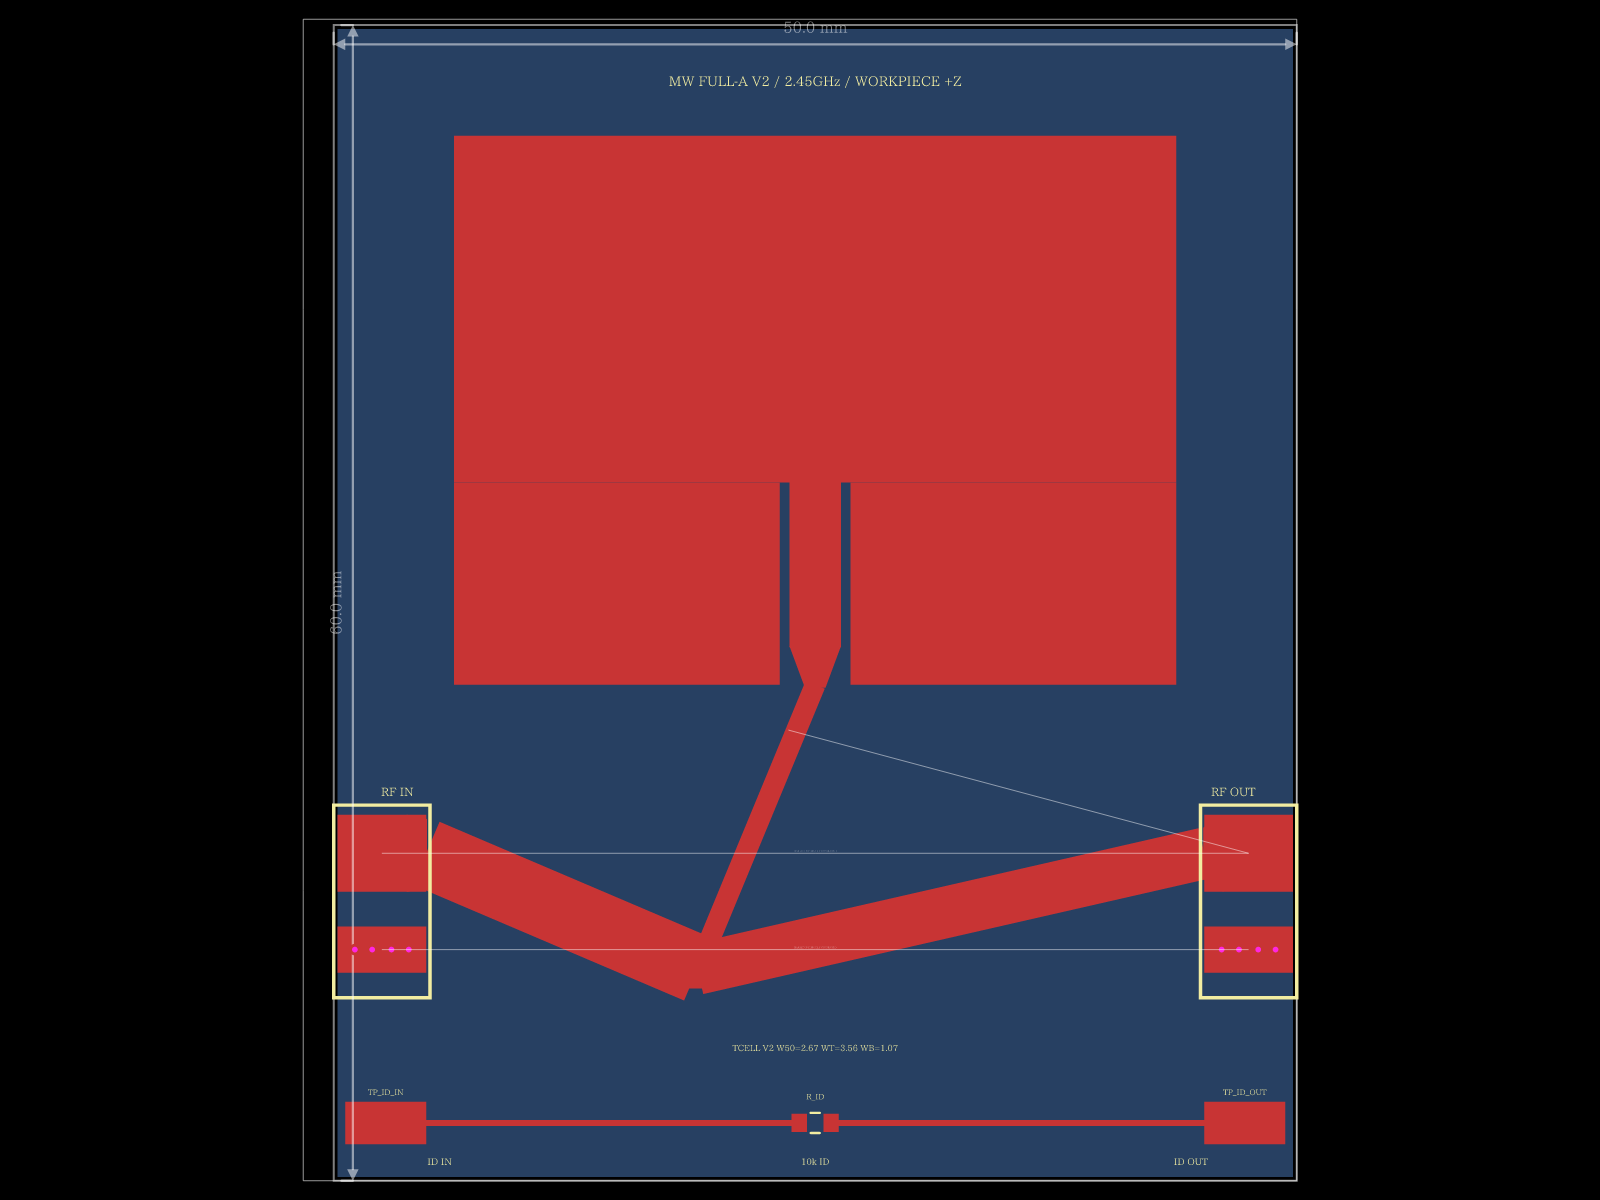
\includegraphics[width=0.72\linewidth]{assets/full-v2-top.png}
  \caption{当前 Full V2 顶层版图。大面积红色区域是矩形 Patch，中央为 T-cell 和分支，底边是 ID 链，左右是 RF 接触区。它是工程候选，不是新规格灰板的最终加工图。}
\end{figure}

\section{关键尺寸与 RF 结构}

\subsection{当前板子的效果和目标差距}

下面只列当前板子已经能回答的事情。目标值放在右列，是为了看差距，不是把需求重新抄一遍。

\begin{tabularx}{\linewidth}{>{\bfseries}p{36mm} X >{\raggedleft\arraybackslash}p{25mm}}
\toprule
观察项 & 当前板子能说明什么 & 距离目标 \\
\midrule
单板匹配 & 2.45 GHz 处 S11 = -19.34 dB，VSWR = 1.242；VSWR<=2 带宽 300 MHz & 已达到 RF 筛选线 \\
RF through & S21 = -12.49 dB；说明 RF 链路仍有明显非 through 功率，但它不是工件吸收 & 不能换算成 5-8 W \\
ID 支路 & off/open/10 kΩ 的变化很小，当前 ID 结构对 RF 影响可忽略 & 已接近目标 \\
加载取能 & 5 mm gap 记录只有 0.182 ns，跨 profile 不稳定 & 尚无有效数值 \\
组内均匀性 & 没有 5、25、100 板串联模型，也没有每板功率分布 & 尚未开始量化 \\
桥接与线缆 & 当前 Full V2 模型未包含两类桥和 5 m 线缆 & 插损差距尚无法量化 \\
\bottomrule
\end{tabularx}

\vspace{3mm}
\statusbox{red}{最重要的判断}{这块板目前证明了“RF 端口和板上拓扑能工作”，还没有证明“每块能稳定取 5-8 W”。从单板 S 参数到 5/25/100 板的功率均匀性，中间还缺加载、桥接、线缆和组态模型。}

\subsection{当前 Full V2 工程参数}

\begin{tabularx}{\linewidth}{>{\bfseries}p{42mm} >{\raggedleft\arraybackslash}p{38mm} X}
\toprule
参数 & 数值 & 说明 \\
\midrule
目标频率 & 2.45 GHz & 当前 RF 设计中心 \\
板框 & 50 mm x 60 mm & 当前机械目标，不是旧版 50 mm x 70 mm \\
Patch & 37.5 mm x 28.5 mm & inset-fed 矩形 Patch \\
50 Ω through 宽度 & 2.670 mm & 当前 surrogate-calibrated 候选 \\
series branch 宽度 & 3.557 mm & 约 42.11 Ω 的变换段 \\
Patch branch 宽度 & 1.073 mm & 约 78.10 Ω 的变换段 \\
T-junction & (-6.1105, -24.0072) mm & 八边形节点，直径 2.2 mm \\
ID 电阻 & 10 kΩ, 0603 & 低频识别链 \\
\bottomrule
\end{tabularx}

\vspace{3mm}
\statusbox{teal}{RF 路径怎么读}{RF IN -> pad taper -> V2 T-cell -> RF OUT；T 点另一路 -> branch taper -> inset feed -> Patch。两个 RF 端口在 openEMS 里采用顶层 signal-to-GND 的 coplanar lumped port，和当前磁吸接触结构一致。}

\section{桥接件和连接线的差距}

这些部件决定了串联组态里每一段到底损失多少。当前板子仿真没有把它们放进去，因此这里不能给“已达到”的判断。

\begin{tabularx}{\linewidth}{>{\bfseries}p{28mm} X >{\raggedleft\arraybackslash}p{25mm}}
\toprule
部件 & 当前证据 & 距离目标 \\
\midrule
平面连接桥 & 没有结构模型、触点模型或插损结果 & 目标 <= 0.2 dB，待建模/测试 \\
立体直角桥 & 没有 L 形走线和直角过渡模型 & 目标 <= 0.3 dB，待建模/测试 \\
5 m 连接线 & 当前 Full V2 没有 N 头、磁吸片或 RG142 模型 & 目标 <= 0.5 dB，待测 \\
组内级联 & 没有 5、25、100 板的逐板功率分布 & 偏差 <= +/-25\%，待建立 \\
\bottomrule
\end{tabularx}

下一版应把两类桥和线缆作为独立 coupon 先测清楚，再把实测或拟合的 S 参数带入 5、25、100 板串联模型。这样得到的才是系统级插损和取能均匀性，不会把单板空载数据误当成整组结果。

\section{PCB 工程检查结果}

这部分是“板子画得对不对”，不是“天线性能好不好”。Full V2 当前检查结果如下：

\begin{itemize}
  \item netlist：0 errors，RF1、ID IN、R\_ID、ID OUT 的连接关系完整；
  \item placement：0 errors，板顶层铜占用约 72.6\%；
  \item 两段 ID 走线：各 21.48 mm，左右对称；
  \item routing difficulty：没有拥塞区域；
  \item build：通过，已生成 circuit JSON、PCB SVG、schematic SVG 和 3D PNG；
  \item shorts：未发现短路。
\end{itemize}

有几条提示不应被忽略。RF1 还没有 courtyard 和完整 pinAttributes，RF1 也没有标出 requires\_power / requires\_ground；0603 电阻的供应商封装在线抓取失败。这些提示没有阻止当前几何 build，但在下单前需要补齐并重新跑一遍制造检查。

\section{空载 RF 结果}

空载结果回答的是：真实板框、launch、T-cell、Patch 和底层地放在一起后，RF 链路有没有明显坏掉。

\begin{tabularx}{\linewidth}{lrrrrr}
\toprule
工况 & S11 (dB) & S21 (dB) & VSWR & VSWR<=2 带宽 & 质量门 \\
\midrule
fast / ID off & -19.371 & -12.484 & 1.241 & 300 MHz & 通过 \\
fast / ID open & -19.338 & -12.491 & 1.242 & 300 MHz & 通过 \\
fast / ID 10 kΩ & -19.339 & -12.491 & 1.242 & 300 MHz & 通过 \\
screen / ID open & -17.153 & -11.688 & 1.322 & 400 MHz & 通过 \\
\bottomrule
\end{tabularx}

这组结果足以支持“继续做加载模型”的决定，但还不是最终加工公差下的精确预测。fast 和 screen 的 S11 相差约 2.2 dB，说明后面还需要用更一致的网格和时窗做 verify。

\section{加载工件：目前不能下什么结论}

当前加载模型是 2 mm front PP + air gap + 有损工件，工件参数取 $\varepsilon_r'=10$、$\tan\delta=0.2$、厚度 20 mm。已有 0、5、10、20 mm gap 的 smoke 记录，也有 5 mm gap 的 loaded/fast 记录。

问题不在于没有数，而在于时域记录太短。同一个 5 mm gap：

\begin{tabularx}{\linewidth}{lrrrr}
\toprule
profile & S11 (dB) & S21 (dB) & 最短时窗 & 判定 \\
\midrule
smoke & -19.236 & -45.140 & 0.318 ns & 不可用 \\
loaded & -33.437 & -85.574 & 0.182 ns & 不可用 \\
fast & -25.014 & -300 & 0.045 ns & 不可用 \\
\bottomrule
\end{tabularx}

所以目前不能把 $1-|S_{11}|^2-|S_{21}|^2$ 写成工件吸收率。这个量还混合了 Patch 辐射、FR4/PP 损耗、边界流出，以及仿真时窗没有覆盖完整响应的问题。报告里保留这些数字，是为了追踪故障，不是为了比较 gap 哪个最好。

\section{制造前还要补什么}

剩下的工作有三块。第一块是灰板本身：把当前 50 mm x 60 mm Full V2 改成目标 50 mm x 50 mm，确认方形螺旋线圈、直通线、耦合段和 ID 走线的相对位置，再检查 PP 外壳、FR4 厚度、磁铁和磷青铜触点的装配余量。

第二块是功率均匀性：先把 5 mm gap 的时域记录拉到至少 1 ns，再做 1 ns、2 ns 的稳定性对比；随后建立 5、25、100 板串联模型，加入桥接件和 5 m 连接线的插损，直接看每块板的输入功率、取能功率和位置偏差。单板空载 S 参数通过，不代表组内 100 块仍然均匀。

第三块是加工和交付：补 RF1 的 courtyard、pin attributes 和 GND 电气属性；固定 0603 封装来源，重新检查 Gerber、阻焊开窗、板边和触点尺寸；最后形成两项交付物，一份带数据和复现命令的仿真报告，以及灰板、平面连接桥、立体直角桥和连接线的优化加工图纸。

\section{文件和复现入口}

\begin{tabularx}{\linewidth}{p{0.43\linewidth} X}
\toprule
文件 & 用途 \\
\midrule
\scriptsize\texttt{pcb/tscircuit/index-full-v2.tsx} & Full V2 PCB 入口 \\
\scriptsize\texttt{pcb/tscircuit/src/full-engineering-board-v2.tsx} & Full V2 版图实现 \\
\shortstack[l]{\scriptsize\texttt{pcb/tscircuit/src/full-engineering-board-v2-}\\[-1pt]\scriptsize\texttt{geometry.json}} & 与 EM 共用的几何参数 \\
\scriptsize\texttt{scripts/openems/simulate\_full\_v2\_fast.py} & Full V2 openEMS 模型和结果后处理 \\
\shortstack[l]{\scriptsize\texttt{docs/30\_full\_v2\_loaded\_simulation\_}\\[-1pt]\scriptsize\texttt{closure\_v1.md}} & 加载仿真闭合审计 \\
\bottomrule
\end{tabularx}

\vspace{4mm}
当前推荐先冻结目标规格和接口尺寸，再把 Full V2 的 50 mm x 60 mm 候选改成 50 mm x 50 mm 灰板版本。之后重跑 5 mm loaded verify 和 5/25/100 板功率均匀性。现有板子能用于工程筛选，但还不该被当成最终生产文件。

\end{document}
